% PROPOSTA------------------------------------------------------------------

\chapter{DESENVOLVIMENTO}
\label{chap:proposta}

\par Este trabalho tem como proposta a construção de um algoritmo para a identificação e descrição de texturas de imagens através da aplicação de árvores geradoras mínimas. Sendo assim, neste capítulo serão esclarecidas as ações tomadas nas diferentes etapas do projeto e as ferramentas utilizadas para a sua execução.

\section{MÉTODO}
\label{sec:metodo}

\par O método de desenvolvimento utilizado possui 6 etapas principais, as quais estão listadas a seguir e se encontram em ordem de execução:

\begin{enumerate}
    \item Selecionar uma imagem;
    \item A partir da imagem, convertê-la em um grafo sem arestas, no qual cada pixel representa um vértice e armazena o seu valor;
    \item Ligar todos os \textit{pixels} com seus vizinhos, caracterizando vizinhança 8, ou 4 caso o \textit{pixel} esteja na borda;
    \item Atribuir valores (pesos) a cada aresta do grafo formado. Este valor corresponde ao módulo da diferença entre os valores do pixel em \textit{8-bits}, ou seja, valores entre 0 e 255;
    \item Encontrar uma árvore geradora mínima do grafo;
    \item Extrair um vetor de características a partir dos valores obtidos em cada aresta da MST. Tal vetor é formado pela: média simples, desvio padrão, grau de assimetria, curtose e entropia.
    % \item Analisar resultado obtido;
    % \item Repetir os passos anteriores com um \textit{dataset} de várias imagens;
    % \item Comparar o algoritmo realizado com outros algoritmos presentes na literatura;
    % \item Analisar resultados obtidos e fazer as devidas modificações e aprimoramentos.
\end{enumerate}

\par A \autoref{fig:metodo} ilustra o método descrito acima, com o intuito de facilitar a compreensão e retratar de forma mais objetiva e concisa. Em seguida, cada etapa será descrita de forma mais detalhada.

\begin{figure}[h]
    \centering
    \caption{Diagrama de etapas do método desenvolvido}
    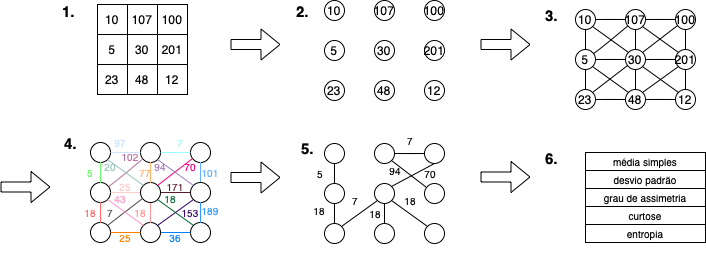
\includegraphics[width=1\textwidth]{./dados/figuras/metodo.png}
    \fonte{Autoria Própria.}
    \label{fig:metodo}
\end{figure}

\par Na etapa 1, é obtida a imagem, onde cada \textit{pixel} contém o seu valor. Na segunda etapa, a imagem é convertida para um grafo, ainda sem arestas, onde cada vértice contém o valor do \textit{pixel}. Já na etapa 3, são feitas todas as ligações possíveis de um vértice com o seus vizinhos, considerando vizinhança-8 ou vizinhança-4, caso o vértice esteja localizado na borda. Na quarta etapa, as arestas são ponderadas, ou seja, são atribuídos valores a estas, sendo esse valor correspondente ao módulo da diferença entre os dois vértices. Na penúltima etapa, é formada a árvore geradora mínima. Por fim, na etapa 6, a partir dos valores das arestas da MST obtida, é formado um vetor por cinco características: média simples, desvio padrão, grau de assimetria, curtose e entropia.
\begin{comment}
\par Por fim, vale ressaltar que este processo poderá ser realizado diversas vezes em uma mesma imagem, de forma a serem obtidas diferentes MST. Isto será possível, de modo que, algumas arestas e vértices serão eliminados propositalmente após a quarta fase, deste modo o que caracterizará a eliminação destes será um valor específico, maior ou menor que um valor empírico obtido durante os experimentos. Além disto, o valor será padronizado com estimativas de média e desvio padrão, antes da sexta etapa, de forma que um mesmo grafo que possua diversas MST não será necessário analisar-se todas as possibilidades, de forma a garantir um vetor de características padronizado.
\end{comment}

%% Parte escrita sobre o cascata-----------------------------------------------
\begin{comment}
\par Para a aplicação do trabalho, será utilizado o modelo cascata como processo de software, como pode ser observado na figura \ref{fig:modelo_cascata}, que representa tal modelo segundo \citeonline{Sommerville2011}. 

\begin{figure}[!h]
    \centering
    \caption{O modelo cascata}
    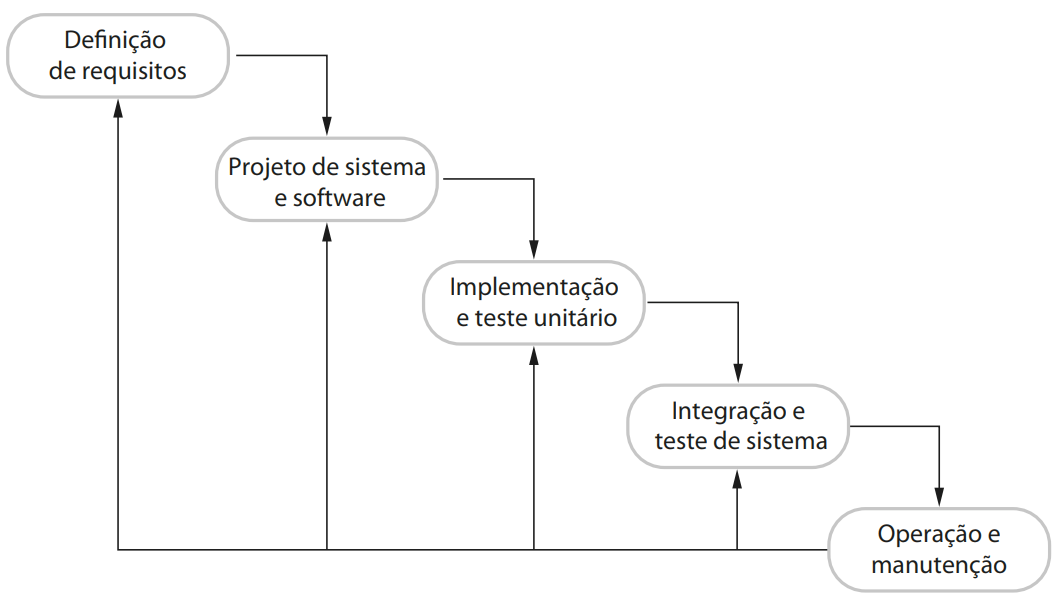
\includegraphics[width=1\textwidth]{./dados/figuras/modelo_cascata.png}
    \fonte{\citeonline{Sommerville2011}}
    \label{fig:modelo_cascata}
\end{figure}
\par Abaixo estão descritas cada fase do processo, que devem ser previamente planejadas e quais seus objetivos a serem cumpridos. Foi utilizado como base o trabalho de \citeonline{Sommerville2011} onde o autor define cada fase e as detalha.
\par Na etapa de comunicação, também conhecida como definição de requisitos, é onde serão elicitados os requisitos funcionais e não funcionais, resultando em uma melhor descrição do programa.
\par No projeto de sistema de software será realizado um planejamento, através do desenvolvimento do cronograma geral. O primeiro cronograma desenvolvido para o projeto pode ser visualizado no capítulo \ref{chap:cronograma} desse trabalho. Também haverá modelagem, a qual vai abordar a construção de alguns diagramas UML, tendo como objetivo maior a validação dos requisitos levantados anteriormente. Além de uma análise da estrutura geral do projeto com diagramas de classes e sequência.
\par A fase de implementação e teste unitário, se refere à construção de pequenos módulos e testes dos mesmos, utilizando das ferramentas e tecnologias anteriormente descritas e tendo como foco os requisitos.
\par Já a integração e teste de sistema é um complemento da fase anterior, onde todos os módulos implementados deverão ser integrados de forma a compor um único programa, o qual deve ser testado.
\par Por fim, a última etapa expõe a entrega final, quando o algoritmo, o documento e a validação devem se encontrar finalizados. No entanto, essa fase também diz a respeito de um \textit{feedback} do orientador, onde serão corrigidos e aprimorados certos módulos.
\end{comment}
%% Fim Parte escrita sobre o cascata-----------------------------------------------

\section{DESENVOLVIMENTO DO ALGORITMO}
\label{sec:desenvolvimentoalgoritmo}

\par A partir do uso das ferramentas, \autoref{sec:tecnologiasferramentas}, da busca pelo alcance dos objetivos descritos na \autoref{subsec:objgerais} e da aplicação do método elaborado, \autoref{sec:metodo}, foi possível desenvolver o algoritmo que será descrito nesta subseção.

\par O algoritmo em si deverá ligar todos os \textit{pixels} com seus vizinhos\footnote{Vizinhança-8 ou vizinhança-4, caso este seja um \textit{pixel} que esteja localizado na borda da imagem.}, o que irá formar um grafo. Cada aresta deste grafo receberá um peso, sendo representado pelo módulo da diferença do \textit{pixel} com o seu vizinho. A partir do grafo formado, utilizando a biblioteca \textit{igraph}, será gerado um segundo grafo correspondente a árvore geradora mínima\footnote{Vale ressaltar que tal MST formada a partir do primeiro grafo, também está contida neste.} a partir dos pesos das arestas.

\subsection{PRIMITIVAS}
\label{subsec:primitivas}

\par O algoritmo desenvolvido busca, a partir de uma imagem digital, descrever e identificar a sua textura, através de MST. Para que fosse possível alcançar o seu objetivo, foram definidas algumas primitivas consideradas para o desenvolvimento, as mesmas estão disponíveis em seguida:

\begin{itemize}
    \item Deve-se utilizar as ferramentas e tecnologias descritas na  \autoref{sec:tecnologiasferramentas};
    \item O algoritmo deve seguir o método presente na \autoref{sec:metodo};
    \item Os pesos das arestas do grafo devem ser um parâmetro de fácil modificação. Isto se torna importante pois possibilita a troca do critério que forma o peso das arestas, o que pode ser usado em outros testes resultando na melhoria do algoritmo e consequentemente em sua manutenção;
    \item Devem ser consideradas somente imagens em formato \textit{png}, imagens em outros formatos podem ser convertidas mantendo aproximadamente o tamanho em \textit{bytes} atual;
    \item Precisam ser consideradas apenas imagens em escala de cinza, utilizando da biblioteca \textit{Scikit-Image} \cite{ScikitImage} para converter imagens que não estiverem em tal escala;
    \item Por fim, devem ser consideradas imagens em \textit{8-bits}, ou seja, que apresentem um valor entre 0 e 255, utilizando também a biblioteca \textit{Scikit-Image} \cite{ScikitImage} para converter imagens quando necessário.
\end{itemize}

\section{TECNOLOGIAS E FERRAMENTAS}
\label{sec:tecnologiasferramentas}

\par Atualmente existem várias ferramentas que podem auxiliar o processamento digital de imagens, sendo uma dessas a \textit{Open Source Computer Vision Library} (OpenCV).
A biblioteca OpenCV é produzida em C++ e atualmente está disponível para uso por linguagens de programação como: python, java, linguagem C e C++ \cite{opencv_library}.

\par Tal biblioteca, aberta à comunidade, possui uma estrutura modular, de forma que alguns de seus módulos sejam: processamento de imagens, análise de vídeo, calibração de câmera e reconstrução em 3D, funcionalidades de \textit{framework} 2D, detecção de objetos, \textit{Graphical User Interface} (GUI) de alto nível, entrada e saída de vídeo, entre outros \cite{opencv_library}.

\par No entanto, este projeto será desenvolvido utilizando a biblioteca Scikit-Image, a qual também é \textit{open-source} e está em constante atualização, como é possível observar em seu GitHub. Esta biblioteca é escrita em python e também é utilizada por programas escritos em python.

\par A Scikit-Image possui várias funções que podem ser facilmente utilizadas, fornecendo rotinas versáteis e intuitivas de processamento digital de imagens, provendo sub-módulos dedicados a: cor, desenho, exposição, análise de texturas e bordas, grafos, entrada e saída, entre tantos outros que indiscutivelmente podem auxiliar a muitos na construção de um \textit{software} destinado a processamento de imagens  \cite{ScikitImage}.

\par A escolha de tal biblioteca foi dada principalmente devido as suas funcionalidades que estão em constante atualização, por ser feita nativamente em python, seu uso ser intuitivo e vários outros aspectos que a tornam mais interessante que a OpenCV para este projeto.

\par Como linguagem de programação, será adotada a linguagem python, pois possui consigo várias vantagens, que podem ser observadas facilmente em seu \textit{website} e GitHub tais como: a vasta coleção de bibliotecas, sendo várias de cunho científico, a possibilidade da escrita de códigos legíveis e sua comunidade presenta na evolução da linguagem, por ser \textit{open-source}.


\par Por fim, será utilizada a biblioteca igraph, que irá auxiliar a construir os grafos para uma determinada imagem e também encontrar a árvore geradora mínima \cite{igraph}. Além da biblioteca scikit-learn a qual será utilizada durante as validações para testar o algoritmo e compará-lo a outros já existentes \cite{scikit-learn}.

\section{VALIDAÇÕES}
\label{sec:validacoes}

\par Assim que o algoritmo tenha atendido todas as primitivas e cumprido com o esperado, será necessário comprovar a sua eficácia. Para isto, o algoritmo será comparado com outros métodos de descrição de imagens, mais especificamente de texturas, já presentes na literatura, sendo estes: Gabor \cite{gaborZhang2000content}, Haralick \cite{haralick1973textural}, \textit{local binary patterns} (LBP) \cite{lbp-guo2010rotation} e Tamura \cite{tamura1978textural}.

\par De modo a comparar os extratores, serão realizados alguns testes com diferentes algoritmos de aprendizado supervisionado, como: \textit{decision tree}, \textit{k-nearest neighbors} (KNN), \textit{linear support vector classification} (\textit{Linear} SVC) e \textit{c-support vector classification} (SVC).

\par Para o algoritmo de aprendizado supervisionado, deve-se manter a semente com um valor igual a 5 (cinco), garantindo que, ao ser executado com as mesmas condições, o algoritmo sempre desempenhe os mesmos resultados. Além disso, deve-se separar o \textit{dataset} em 20\% teste e 80\% treino, ser capaz de ler arquivos em formato \textit{attribute-relation file format} (ARFF) e \textit{comma-separated values} (CSV).

\par Dessa forma, os resultados devem ser salvos para consulta posterior e apresentar: acurácia, precisão, \textit{recall}, \textit{f-score}, matriz de confusão e relatório de classificação por classes. Assim, as acurácias obtidas pelos extratores serão comparadas quando testados com diferentes algoritmos de aprendizado supervisionado, além da análise da matriz de confusão. Por fim, será calculado o tempo de execução dos extratores.

\begin{comment}
\par Além disso, serão utilizados algoritmos de classificação supervisionada para apresentar taxas de acerto, eficácia e a eficiência.

\par Como variável de comparação será primeiramente utilizada a capacidade do código de descrever a textura de uma imagem, quando comparado a outros algoritmos bem aceitos pela comunidade científica, os quais também foram citados anteriormente. Dessa forma, serão analisados entre os algoritmos, quais são capazes de oferecer o melhor resultado final, ou seja, a partir de uma imagem, sejam capazes de apresentar dados da textura e suas características.

\par Com o uso da biblioteca \textit{scikit-learn}, é esperado como resultado final uma taxa de acurácia e uma análise da matriz de confusão da comparação entre os procedimentos.

\par Além disso, também será comparada, porém em segunda instância, o custo computacional dos algoritmos. Sendo tomado vez o tempo de execução e vez o uso de memória primária e processamento. Esta validação será considerada principal caso a outra validação mostre que o algoritmo não obteve um resultado satisfatório, porém pode ser levado em consideração caso este se mostre mais eficiente que outros nestes aspectos.

\par Por fim, vale ressaltar que serão utilizadas as seguintes bases de dados: Vison Texture Database (VisTex) \cite{vistex} e a USPTex \cite{usptex}.
\end{comment}

\subsection{DATASETS}
\label{subsec:datasets}

\par Para testar o algoritmo são necessárias imagens, para isto alguns \textit{datasets} fornecem uma quantidade vasta de imagens que são dividas em grupos. Dessa forma, foram escolhidos quatro \textit{datasets} com foco para testar a característica de textura de algoritmos de extração de características.

\subsubsection{USC-SIPI TEXTURES}
\label{subsubsec:usc-spi}

\par O USC-SIPI \textit{Textures} \cite{weber1997usc} é um \textit{dataset} composto por um conjunto de imagens, entre essas algumas extraídas do \textit{dataset} Brodatz \cite{brodatz1966textures}, o qual segundo \citeonline{fekri2019new}, é formado através de fotografias digitalizadas para diversos propósitos, o que o torna um dos mais populares.
\par O \textit{dataset} possui somente imagens monocromáticas, \textit{8-bits}, sendo a resolução de 130 destas 512x512 \textit{pixels} e 25 de 1024x1024 \textit{pixels}, totalizando 155 imagens. No entanto, para a validação foi utilizado o \textit{dataset} com imagens rotacionadas em sete graus diferentes: 0, 30, 60, 90, 120, 150 e 200 graus, totalizando 91 imagens de 512x512 \textit{pixels}. Este \textit{dataset} possui um total de 13 classes, alguns exemplos de imagens podem ser observados na \autoref{fig:usc-sipi} \cite{weber1997usc}. Por fim, suas classes são: \textit{Bark}, \textit{Brick}, \textit{Bubbles}, \textit{Grass}, \textit{Leather}, \textit{Pigskin}, \textit{Raffia}, \textit{Sand}, \textit{Straw},
\textit{Water}, \textit{Weave}, \textit{Wood}, \textit{Wool} \cite{weber1997usc}.

\begin{figure}[!h]
    \centering
    \caption{Exemplos de imagens disponíveis no \textit{dataset} USC-SIPI \textit{Textures}}
    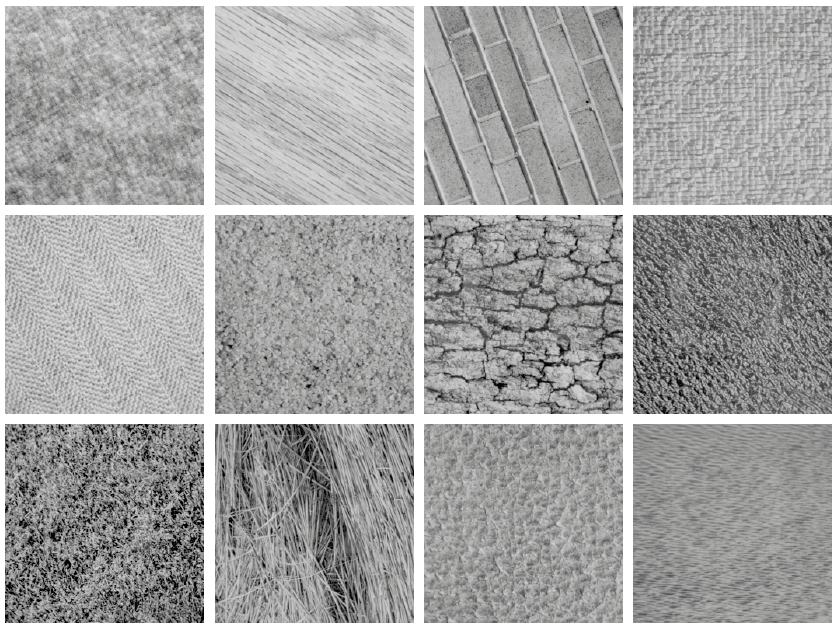
\includegraphics[width=0.7\textwidth]{./dados/figuras/usc-sipi.png}
    \fonte{\citeonline{weber1997usc}.}
    \label{fig:usc-sipi}
\end{figure}

% KYBERG
\subsubsection{KYLBERG}
\label{subsubsec:kylberg}

\par Segundo \citeonline{Kylberg2011c}, seu \textit{dataset} possui 28 classes, sendo que cada uma possui 160 imagens em resolução 576x576 \textit{pixels}, \textit{8-bits} e formato PNG. Além de todas imagens serem normalizadas com desvio padrão correspondendo a 40 e um valor médio de 127. A \autoref{fig:kylberg} apresenta algumas imagens pertencentes a este \textit{dataset}.

\begin{figure}[!h]
    \centering
    \caption{Exemplos de imagens disponíveis no \textit{dataset} Kylberg}
    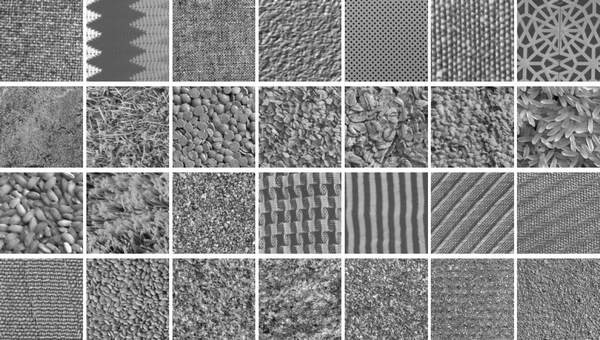
\includegraphics[width=0.7\textwidth]{./dados/figuras/kylberg.jpg}
    \fonte{\citeonline{Kylberg2011c}.}
    \label{fig:kylberg}
\end{figure}


\subsubsection{USPTEX}
\label{subsubsec:usptex}

\par Este \textit{dataset} possui um total de 2.292 imagens, dividas em 191 classes, todas com resolução de 128x128 \textit{pixels}, apesar das imagens originais estarem em 512x512 \textit{pixels}. Estas possuem texturas com cores naturais adquiridas sob uma fonte de luz fixa desconhecida. Alguns exemplos destas em sua forma original estão disponibilizados na \autoref{fig:usptex} \cite{usptex}. Vale ressaltar, que tal \textit{dataset} teve suas imagens convertidas em escala de cinza para utilização neste trabalho.

\begin{figure}[!h]
    \centering
    \caption{Exemplos de imagens disponíveis no USPtex}
    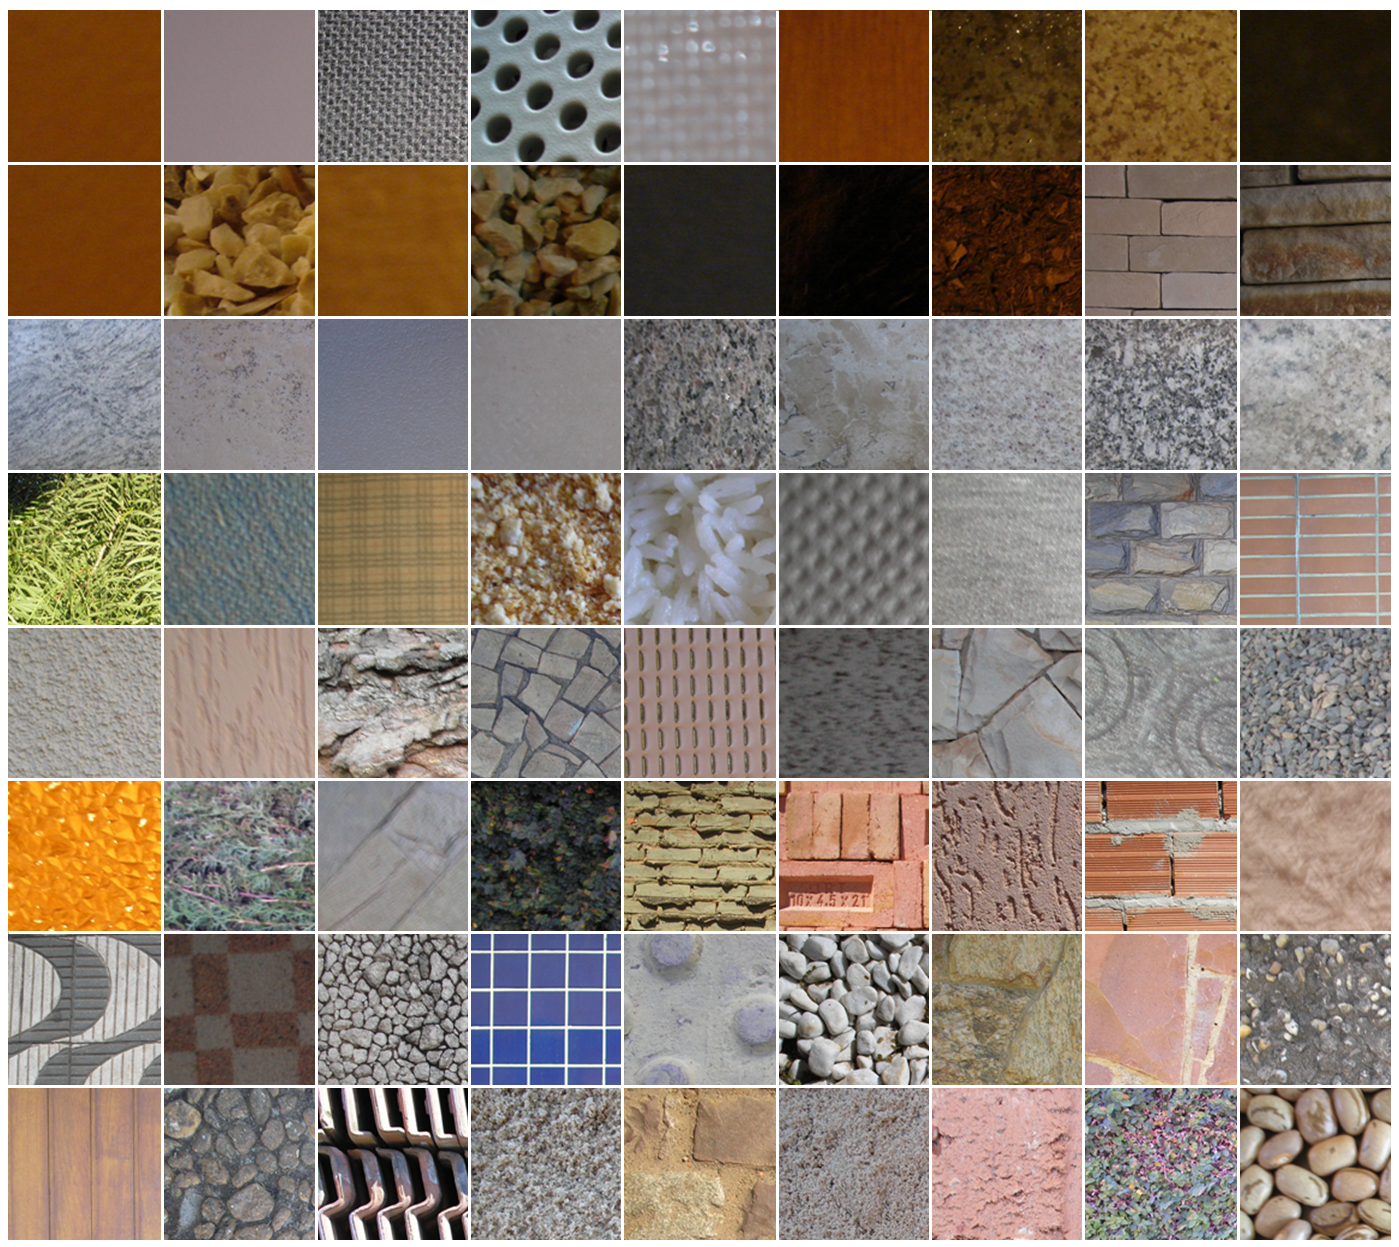
\includegraphics[width=0.7\textwidth]{./dados/figuras/USPtex.png}
    \fonte{\citeonline{usptex}.}
    \label{fig:usptex}
\end{figure}

\subsubsection{VISTEX}
\label{subsubsec:vistex}

\par O \textit{Vision Texture} (VisTex), é um \textit{dataset} que provem uma quantia vasta de texturas de alta qualidade para aplicação em contextos de visão computacional. Dessa forma, as imagens retratam o mundo real e oferecem texturas tanto tradicionais quanto não tão tradicionais \cite{vistex}. Estas imagens são coloridas e possuem uma resolução de 128x128 \textit{pixels} e um total de 40 classes \cite{fekri2019new}. Para os testes foram consideradas 19 classes, totalizando 167 imagens, também transformadas em escala de cinza. A \autoref{fig:vistex} expõe algumas exemplos deste \textit{dataset} utilizados nas validações.

\begin{figure}[H]
    \centering
    \caption{Exemplos de imagens disponíveis no VisTex}
    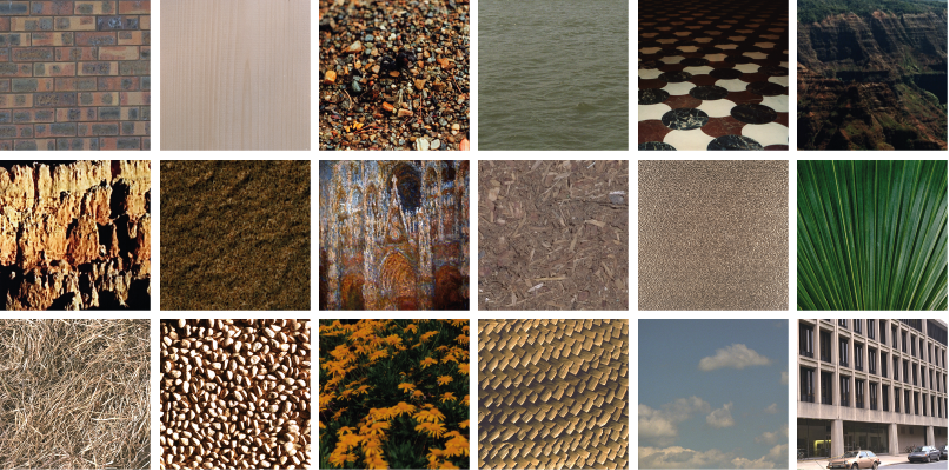
\includegraphics[width=0.7\textwidth]{./dados/figuras/vistex.png}
    \fonte{\citeonline{vistex}.}
    \label{fig:vistex}
\end{figure}

\begin{comment} 
\section{CRONOGRAMA}
\label{sec:cronograma}

\par Este capítulo tem como objetivo apresentar um cronograma para o futuro deste projeto. As fases, bem como suas atividades estão listadas logo em seguida e podem ser melhor observadas por meio da \autoref{tab:cronograma} e também através da \autoref{tab:cronograma-fases} as quais fazem uma relação entre atividades, fases e datas.

Vale ressaltar que as tabelas apresentam um mês e logo abaixo o número 1 e 2, o número 1 faz referência à primeira metade do mês e o número 2 à segunda metade\footnote{Exemplo: Dado o mês de novembro, o número 1 faz referência do dia 1 ao 15, já o número 2 faz referência do dia 16 ao 30.}.


\begin{enumerate}
    \item Correções
        \begin{enumerate}
            \item[1.1] Fazer as devidas correções neste documento, conforme detalhes apresentados pela banca e pelo orientador;
            \item[1.2] Verificar e validar correções.
        \end{enumerate}

    \item Preparação
        \begin{enumerate}
            \item[2.1] Definir premissas;
            \item[2.2] Definir módulos;
            \item[2.3] Verificar e validar;
            \item[2.4] Documentar e escrever sobre esta fase.
        \end{enumerate}

    \item Implementação
        \begin{enumerate}
            \item[3.1] Aprofundar conhecimentos em linguagem \textit{python};
            \item[3.2] Estudar novamente a documentação das bibliotecas e demais ferramentas, focando nos métodos que serão utilizados;
            \item[3.3] Iniciar a programação módulo $n$;
            \item[3.4] Testar o módulo $n$;
            \item[3.5] Documentar e escrever sobre esta fase.
        \end{enumerate}
        
    \item Integração
        \begin{enumerate}
            \item[4.1] Integrar os módulos da fase anterior;
            \item[4.2] Testar a integração;
            \item[4.3] Preparar o teste para a validação do algoritmo;
            \item[4.4] Testar o algoritmo;
            \item[4.5] Documentar e escrever sobre esta fase.
        \end{enumerate}
        
    \item Testes e comparações
        \begin{enumerate}
            \item[5.1] Estudar outros algoritmos de descrição de imagens;
            \item[5.2] Preparar testes entre o algoritmo obtido na fase anterior com os presentes na literatura;
            \item[5.3] Realizar testes;
            \item[5.4] Analisar resultados;
            \item[5.5] Verificar e validar;
            \item[5.6] Documentar e escrever sobre esta fase.
        \end{enumerate}
    
    \item Operação e manutenção
        \begin{enumerate}
            \item[6.1] Observar os resultados da etapa anterior e fazer as devidas modificações para a melhor eficiência do algoritmo;
            \item[6.2] Documentar e escrever sobre esta fase.
        \end{enumerate}
        
    \item Documentação
        \begin{enumerate}
            \item[7.1] Finalizar o documento referente ao Trabalho de Conclusão de Curso 2, utilizando da documentação das fases anteriores, além do documento produzido para o Trabalho de Conclusão de Curso 1;
            \item[7.2] Preparar apresentação.
        \end{enumerate}
        
\end{enumerate}

% Please add the following required packages to your document preamble:
% \usepackage[table,xcdraw]{xcolor}
% If you use beamer only pass "xcolor=table" option, i.e. \documentclass[xcolor=table]{beamer}
\begin{table}[H]
\centering
\caption{Cronograma do projeto por atividades.}
\label{tab:cronograma}
\resizebox{\textwidth}{!}{
\begin{tabular}{|l|l|l|l|l|l|l|l|l|l|l|l|l|l|l|l|l|}
\hline
\multicolumn{17}{|c|}{Cronograma}                                                                                                                                                                                                                                                                                                                                                                                                                                                                                                                     \\ \hline
Ano       & \multicolumn{4}{c|}{2019}                                                                                                        & \multicolumn{12}{c|}{2020}                                                                                                                                                                                                                                                                                                                                                                             \\ \hline
Mês       & \multicolumn{2}{c|}{Novembro}                                              & \multicolumn{2}{c|}{Dezembro}                       & \multicolumn{2}{c|}{Janeiro}                        & \multicolumn{2}{c|}{Fevereiro}                      & \multicolumn{2}{c|}{Março}                                                                        & \multicolumn{2}{c|}{Abril}                                                 & \multicolumn{2}{c|}{Maio}                           & \multicolumn{2}{c|}{Junho}                          \\ \hline
Atividade & \multicolumn{1}{c|}{1}   & \multicolumn{1}{c|}{2}                          & \multicolumn{1}{c|}{1}   & \multicolumn{1}{c|}{2}   & \multicolumn{1}{c|}{1}   & \multicolumn{1}{c|}{2}   & \multicolumn{1}{c|}{1}   & \multicolumn{1}{c|}{2}   & \multicolumn{1}{c|}{1}                          & \multicolumn{1}{c|}{2}                          & \multicolumn{1}{c|}{1}                          & \multicolumn{1}{c|}{2}   & \multicolumn{1}{c|}{1}   & \multicolumn{1}{c|}{2}   & \multicolumn{1}{c|}{1}   & \multicolumn{1}{c|}{2}   \\ \hline
1.1       & \cellcolor[HTML]{000000} &                                                 &                          &                          &                          &                          &                          &                          &                                                 &                                                 &                                                 &                          &                          &                          &                          &                          \\ \hline
1.2       & \cellcolor[HTML]{000000} &                                                 &                          &                          &                          &                          &                          &                          &                                                 &                                                 &                                                 &                          &                          &                          &                          &                          \\ \hline
2.1       &                          & \cellcolor[HTML]{000000}{\color[HTML]{000000} } &                          &                          &                          &                          &                          &                          &                                                 &                                                 &                                                 &                          &                          &                          &                          &                          \\ \hline
2.2       &                          & \cellcolor[HTML]{000000}                        &                          &                          &                          &                          &                          &                          &                                                 &                                                 &                                                 &                          &                          &                          &                          &                          \\ \hline
2.3       &                          & \cellcolor[HTML]{000000}                        &                          &                          &                          &                          &                          &                          &                                                 &                                                 &                                                 &                          &                          &                          &                          &                          \\ \hline
2.4       &                          & \cellcolor[HTML]{000000}                        &                          &                          &                          &                          &                          &                          &                                                 &                                                 &                                                 &                          &                          &                          &                          &                          \\ \hline
3.1       &                          &                                                 & \cellcolor[HTML]{000000} &                          &                          &                          &                          &                          &                                                 &                                                 &                                                 &                          &                          &                          &                          &                          \\ \hline
3.2       &                          &                                                 & \cellcolor[HTML]{000000} &                          &                          &                          &                          &                          &                                                 &                                                 &                                                 &                          &                          &                          &                          &                          \\ \hline
3.3       &                          &                                                 & \cellcolor[HTML]{000000} & \cellcolor[HTML]{000000} & \cellcolor[HTML]{000000} & \cellcolor[HTML]{000000} &                          &                          &                                                 &                                                 &                                                 &                          &                          &                          &                          &                          \\ \hline
3.4       &                          &                                                 & \cellcolor[HTML]{000000} & \cellcolor[HTML]{000000} & \cellcolor[HTML]{000000} & \cellcolor[HTML]{000000} &                          &                          &                                                 &                                                 &                                                 &                          &                          &                          &                          &                          \\ \hline
3.5       &                          &                                                 &                          &                          &                          & \cellcolor[HTML]{000000} &                          &                          &                                                 &                                                 &                                                 &                          &                          &                          &                          &                          \\ \hline
4.1       &                          &                                                 &                          &                          &                          &                          & \cellcolor[HTML]{000000} &                          &                                                 &                                                 &                                                 &                          &                          &                          &                          &                          \\ \hline
4.2       &                          &                                                 &                          &                          &                          &                          & \cellcolor[HTML]{000000} &                          &                                                 &                                                 &                                                 &                          &                          &                          &                          &                          \\ \hline
4.3       &                          &                                                 &                          &                          &                          &                          & \cellcolor[HTML]{000000} &                          &                                                 &                                                 &                                                 &                          &                          &                          &                          &                          \\ \hline
4.4       &                          &                                                 &                          &                          &                          &                          & \cellcolor[HTML]{000000} &                          &                                                 &                                                 &                                                 &                          &                          &                          &                          &                          \\ \hline
4.5       &                          &                                                 &                          &                          &                          &                          & \cellcolor[HTML]{000000} &                          &                                                 &                                                 &                                                 &                          &                          &                          &                          &                          \\ \hline
5.1       &                          &                                                 &                          &                          &                          &                          &                          & \cellcolor[HTML]{000000} &                                                 &                                                 &                                                 &                          &                          &                          &                          &                          \\ \hline
5.2       &                          &                                                 &                          &                          &                          &                          &                          & \cellcolor[HTML]{000000} &                                                 &                                                 &                                                 &                          &                          &                          &                          &                          \\ \hline
5.3       &                          &                                                 &                          &                          &                          &                          &                          &                          & \cellcolor[HTML]{000000}{\color[HTML]{000000} } &                                                 &                                                 &                          &                          &                          &                          &                          \\ \hline
5.4       &                          &                                                 &                          &                          &                          &                          &                          &                          & \cellcolor[HTML]{000000}{\color[HTML]{000000} } &                                                 &                                                 &                          &                          &                          &                          &                          \\ \hline
5.5       &                          &                                                 &                          &                          &                          &                          &                          &                          & \cellcolor[HTML]{000000}{\color[HTML]{000000} } &                                                 &                                                 &                          &                          &                          &                          &                          \\ \hline
5.6       &                          &                                                 &                          &                          &                          &                          &                          &                          & \cellcolor[HTML]{000000}{\color[HTML]{000000} } &                                                 &                                                 &                          &                          &                          &                          &                          \\ \hline
6.1       &                          &                                                 &                          &                          &                          &                          &                          &                          &                                                 & \cellcolor[HTML]{000000}{\color[HTML]{000000} } & \cellcolor[HTML]{000000}{\color[HTML]{000000} } & \cellcolor[HTML]{000000} & \cellcolor[HTML]{000000} &                          &                          &                          \\ \hline
6.2       &                          &                                                 &                          &                          &                          &                          &                          &                          &                                                 & \cellcolor[HTML]{000000}{\color[HTML]{000000} } & \cellcolor[HTML]{000000}{\color[HTML]{000000} } & \cellcolor[HTML]{000000} & \cellcolor[HTML]{000000} &                          &                          &                          \\ \hline
7.1       &                          &                                                 &                          &                          &                          &                          &                          &                          &                                                 &                                                 &                                                 & \cellcolor[HTML]{000000} & \cellcolor[HTML]{000000} & \cellcolor[HTML]{000000} & \cellcolor[HTML]{000000} &                          \\ \hline
7.2       &                          &                                                 &                          &                          &                          &                          &                          &                          &                                                 &                                                 &                                                 &                          &                          & \cellcolor[HTML]{000000} & \cellcolor[HTML]{000000} & \cellcolor[HTML]{000000} \\ \hline
\end{tabular}
}
\end{table}

Uma visão mais resumida e menos detalhada pode ser vista na \autoref{tab:cronograma-fases}, estando esta organizada através das fases do projeto, definidas no início desta \autoref{sec:cronograma}.

% Please add the following required packages to your document preamble:
% \usepackage[table,xcdraw]{xcolor}
% If you use beamer only pass "xcolor=table" option, i.e. \documentclass[xcolor=table]{beamer}
\begin{table}[H]
\centering
\caption{Cronograma do projeto por fases.}
\label{tab:cronograma-fases}
\resizebox{\textwidth}{!}{
\begin{tabular}{|l|l|l|l|l|l|l|l|l|l|l|l|l|l|l|l|l|}
\hline
\multicolumn{17}{|c|}{Cronograma}                                                                                                                                                                                                                                                                                                                                                                                                                    \\ \hline
Ano  & \multicolumn{4}{c|}{2019}                                                                                 & \multicolumn{12}{c|}{2020}                                                                                                                                                                                                                                                                                                        \\ \hline
Mês  & \multicolumn{2}{c|}{Novembro}                       & \multicolumn{2}{c|}{Dezembro}                       & \multicolumn{2}{c|}{Janeiro}                        & \multicolumn{2}{c|}{Fevereiro}                      & \multicolumn{2}{c|}{Março}                          & \multicolumn{2}{c|}{Abril}                          & \multicolumn{2}{c|}{Maio}                           & \multicolumn{2}{c|}{Junho}                          \\ \hline
Fase & \multicolumn{1}{c|}{1}   & \multicolumn{1}{c|}{2}   & \multicolumn{1}{c|}{1}   & \multicolumn{1}{c|}{2}   & \multicolumn{1}{c|}{1}   & \multicolumn{1}{c|}{2}   & \multicolumn{1}{c|}{1}   & \multicolumn{1}{c|}{2}   & \multicolumn{1}{c|}{1}   & \multicolumn{1}{c|}{2}   & \multicolumn{1}{c|}{1}   & \multicolumn{1}{c|}{2}   & \multicolumn{1}{c|}{1}   & \multicolumn{1}{c|}{2}   & \multicolumn{1}{c|}{1}   & \multicolumn{1}{c|}{2}   \\ \hline
1    & \cellcolor[HTML]{000000} &                          &                          &                          &                          &                          &                          &                          &                          &                          &                          &                          &                          &                          &                          &                          \\ \hline
2    &                          & \cellcolor[HTML]{000000} &                          &                          &                          &                          &                          &                          &                          &                          &                          &                          &                          &                          &                          &                          \\ \hline
3    &                          &                          & \cellcolor[HTML]{000000} & \cellcolor[HTML]{000000} & \cellcolor[HTML]{000000} & \cellcolor[HTML]{000000} &                          &                          &                          &                          &                          &                          &                          &                          &                          &                          \\ \hline
4    &                          &                          &                          &                          &                          &                          & \cellcolor[HTML]{000000} &                          &                          &                          &                          &                          &                          &                          &                          &                          \\ \hline
5    &                          &                          &                          &                          &                          &                          &                          & \cellcolor[HTML]{000000} & \cellcolor[HTML]{000000} &                          &                          &                          &                          &                          &                          &                          \\ \hline
6    &                          &                          &                          &                          &                          &                          &                          &                          &                          & \cellcolor[HTML]{000000} & \cellcolor[HTML]{000000} & \cellcolor[HTML]{000000} & \cellcolor[HTML]{000000} &                          &                          &                          \\ \hline
7    &                          &                          &                          &                          &                          &                          &                          &                          &                          &                          &                          & \cellcolor[HTML]{000000} & \cellcolor[HTML]{000000} & \cellcolor[HTML]{000000} & \cellcolor[HTML]{000000} & \cellcolor[HTML]{000000} \\ \hline
\end{tabular}
}
\end{table}
\end{comment}

\begin{comment}
\section{CONSIDERAÇÕES FINAIS}
\label{sec:consideracoesFinais}

\par Por tanto, a proposta deste trabalho é definir e especificar um projeto que procura desenvolver uma nova maneira, de descrever texturas em uma imagem, por meio da utilização de grafos e também de árvores geradoras mínimas.
\par Como observado, a descrição é uma parte importante do processamento digital de imagens, pois é capaz de identificar padrões em um objeto selecionado pela etapa de segmentação.
\par Sendo assim, é esperado que com a conclusão do algoritmo, este seja capaz de descrever texturas em imagens digitais de forma a ser mais eficaz e/ou eficiente quando comparado a outros algoritmos já presentes na literatura. Além disso, espera-se que com este documento, devidamente atualizado após a conclusão, possa ser utilizado para futuras melhorias no algoritmo e também em novas abordagens.
\end{comment}

